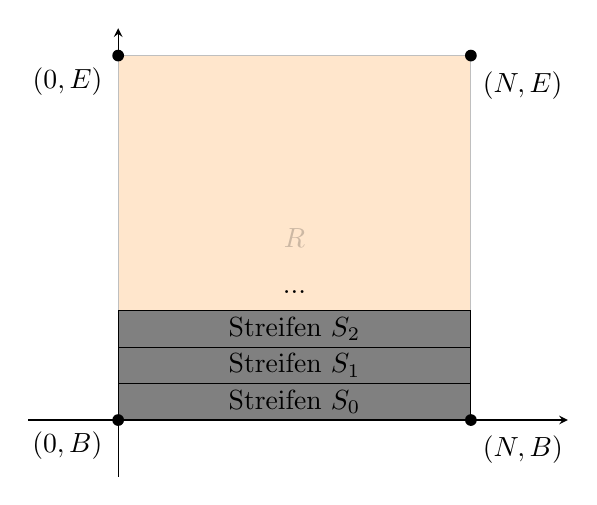
\begin{tikzpicture} 
\begin{axis}[
		ticks=none,
        xmin =-2.55,
        xmax = 12.75,
        ymax = 10.75,
        ymin = -1.55,
        axis x line = middle, axis y line = middle,
        every axis plot/.append style={ultra thick}]

	\draw [draw=lightgray, fill=orange, fill opacity=0.2] (0,0) rectangle node {$R$} (10, 10);
	\draw [fill = gray] (0,0) rectangle node {Streifen $S_0$} (10, 1) ;
	\draw [fill = gray] (0,1) rectangle node {Streifen $S_1$} (10, 2) ;
	\draw [fill = gray] (0,2) rectangle node {Streifen $S_2$} (10, 3) ;
	\node at (5,3.5) {...};
	\node[label={200:{$(0, B)$}},circle,fill,inner sep=1.5pt] at (axis cs:0,0) {};
	\node[label={290:{$(N, B)$}},circle,fill,inner sep=1.5pt] at (axis cs:10,0) {};
	\node[label={200:{$(0, E)$}},circle,fill,inner sep=1.5pt] at (axis cs:0,10) {};
	\node[label={290:{$(N, E)$}},circle,fill,inner sep=1.5pt] at (axis cs:10,10) {};
	%\draw [fill = yellow] (0,7) rectangle node {} (5.26, 10) ;
\end{axis} 
\end{tikzpicture}